\chapter{Lecture}\label{part4:lec36} %%% 36
\markboth{\thechapter. Lecture}{\thechapter. Lecture}

We\pageoriginale were discussing Gaussian sums and it remained to
evaluate
$$
G(h, p) = \left(\frac{h}{p}\right) G(1, p)
$$

We shall do a little more than that; we shall study them in a more
flexible form. Define
$$
S(h, k) = \sum^{k-1}_{\ell =0} e^{\pi i \frac{hg}{k} \ell^2},
$$
$h, k> 0$ but not necessarily coprime. We cannot now take the
summation over $\ell $ modulo $k$. For if $k$ is odd, $(\ell +k)^2=
\ell^2 + 2 \ell k+ k^2$ and $k^2$ may give rise to an odd multiple of
$\pi i$ in the exponent and hence introduce a change of sign, We
should therefore insist on this particular range of summation. $S (h,
k)$ are connected with the Gaussian sums; indeed
$$
G(h, k)= S(2h, k)
$$

We shall now produce $S(h, k)$ as a sum of residues. To get the
integers as poles we should clearly take $e^{2 \pi i \mathfrak{z}}-1$
in the denominator; so we integrate $e^{\pi i \frac{h}{k}
  \mathfrak{z}^2/(e^{2 \pi i \mathfrak{z}}-1)}$ over such a contour as
has in its interior the desired poles $\mathfrak{z} =0, 1, 2, \ldots ,
k-1$. Indeed 
$$
S(h, k)= \int_C \frac{e^{\pi i \frac{h}{k} \mathfrak{z}^2}}{e^{2 \pi i
  \mathfrak{z}}-1} d \mathfrak{z}
$$
\begin{figure}[H]
  \centering{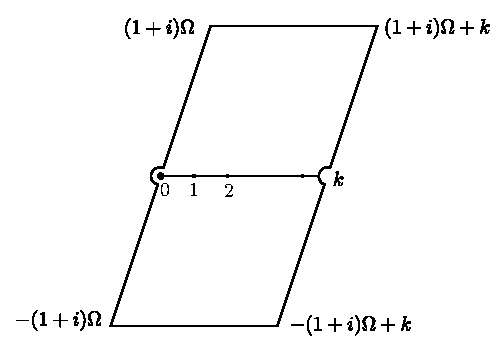
\includegraphics{vol2-figures/fig2.41.eps}}
\end{figure}
Where\pageoriginale $C$ is the parallelogram with vertices at $\pm (1+ i) \Omega$,
$\pm (1+i) \Omega + k$, with the slant sides inclined at $45^\circ$
(infact this may be anything less than $90^\circ$) to the real axis,
and making a detour round 0 and $k$. When we push $\Omega$ to $\infty$,
the integrals along the horizontal sides will tend to zero. For
instance on the upper side, $\mathfrak{z} = (1+i) \Omega +x$, $0 \leq
x \leq k$, and the integrand is therefore
\begin{align*}
  \frac{e^{\pi i \frac{h}{k} ((1+i) \Omega +x)^2}}{e^{2 \pi i ((1+i)
    \Omega +x)}-1} & = \frac{e^{\pi i \frac{h}{k} (2i \Omega^2 + 2(1+i)
    \Omega x+ x^2)}}{e^{2 \pi i (\Omega +x)-2 \pi \Omega}-1}\\
  & = \frac{e^{- \pi \frac{h}{k} (2 \Omega^2 + 2 \Omega x) + \pi i
      \frac{h}{k} (2 \Omega x + x^2)}}{e^{- 2 \pi \Omega + 2 \pi i
      (\Omega +x)}-1}
\end{align*}
$\to 0$\pageoriginale uniformly as $\Omega \to \infty$ since $\frac{h}{k} >
0$. Hence the integral can be written as
$$
\int\limits^{(1+i) \infty+k}_{- (1+i)\infty +k}- \int\limits_{-
  (1+i)\infty}^{(1+i)\infty}  \frac{e^{\pi i \frac{h}{k}
  (\mathfrak{z})^2}}{e^{2 \pi  \mathfrak{z}}-1} d \mathfrak{z} 
$$
where, of course, we have to make a small detour round 0 and
$k$. Replacing $\mathfrak{z}$ by $\mathfrak{z}+k$ in the first
integral, this becomes 
\begin{align*}
  \int\limits_{-(1+i)\infty}^{(1+i)\infty} \frac{e^{\pi i \frac{h}{k}
    (\mathfrak{z}+ k)^2}- e^{\pi i \frac{h}{k} \mathfrak{z}^2}}{e^{2
    \pi i \mathfrak{z}}-1} d \mathfrak{z} 
  & = \int\limits_{-(1+i)\infty}^{(1+i)\infty} \frac{e^{\pi i
    \frac{h}{k}\mathfrak{z}^2}\left(e^{\pi i \frac{h}{k} (2
      \mathfrak{z} k+ k^2)}-1 \right)}{e^{2 \pi i \mathfrak{z}}-1} d
  \mathfrak{z} \\
  & = \int\limits_{-(1+i)\infty}^{(1+i)\infty} \frac{e^{\pi
      \frac{h}{k} \mathfrak{z}^2 \left(e^{2 \pi i h \mathfrak{z} + \pi
      i hk}-1 \right)}}{e^{2 \pi i \mathfrak{z}}-1} d \mathfrak{z}
\end{align*}

Let\pageoriginale us assume from now on that $hk$ is even. Then we can actually
divide out and the integral becomes 
$$
\int\limits_{- (1+i)\infty}^{(1+i)\infty} \left(e^{\pi i
  \frac{h}{k}\mathfrak{z}^2} \sum^{h-1}_{\lambda=0} e^{2 \pi i \lambda
\mathfrak{z}} \right) d \mathfrak{z} 
$$

The denominator has now disappeared. There is a further advantage that
the integral can now be stretched along the whole line and the detour
can be avoided. We then have
$$
\sum^{h-1}_{\lambda=0} e^{-\pi i \lambda^2 \frac{h}{k}}
  \int\limits^{(1+i)\infty}_{- (1+i)\infty} e^{\pi i \frac{h}{k}
    \left( \mathfrak{z}+ \frac{\lambda k}{h}\right)^2} d \mathfrak{z}  
$$

Write $\mathfrak{z} + \lambda k/h= \omega$; and shift the integral
back to the line from $- (1+i)\infty$ to $(1+i)\infty$ - this we can
do since the integrand tends to zero along a horizontal segment. This
gives
$$
\sum^{h-1}_{\lambda =0} e^{- \pi i \frac{h}{k}
  \lambda^2} \int\limits^{(1+i)\infty}_{- (1+i)\infty} e^{\pi i
  \frac{h}{k} \omega^2} d \omega,
$$ 
or\pageoriginale writing $t= \omega \sqrt{\frac{h}{k}}, \sqrt{\frac{h}{k}} > 0$,
$$
\sqrt{\frac{k}{h}} \sum^{h-1}_{\lambda=0} e^{- \pi i \frac{h}{k}
  \lambda^2} \int\limits^{(1+i)\infty}_{-(1+i)\infty} e^{\pi i t^2}
dt= A \sqrt{\frac{k}{h}} \sum^{h-1}_{\lambda=0} e^{- \pi i \frac{k}{h}
\lambda^2} 
$$
where $A$ is the specific constant:
$$
A= \int\limits^{(1+i)\infty}_{-(1+i)\infty} e^{\pi i t^2} dt
$$

Hence 
$$
S(h, k) = A \sqrt{\frac{k}{h}} S(-k, h).
$$

In order to evaluate $A$, take a simple case: $h=1$, $k=2$
$$
\displaylines{S(1, 2)= A \sqrt{2} S(-2, 1)\cr
  \text{i.e.,} \hfill 1+ e^{\frac{\pi i}{2}} = A \sqrt{2}, \hfill }
$$

So $A = (1+i)/ \sqrt{2}$, an eighth root or unity.

So our reciprocity formula becomes complete:
$$
S(h, k)= \frac{1+i}{\sqrt{2}} \sqrt{\frac{k}{h}} S(-k, h).
$$

Let us develop some corollaries.

1)\pageoriginale $h=2$, $k$ arbitrary:
\begin{align*}
  & ~~~~S (2, k)  = G(1, k), ~\text{so}\\
  G(1, k) & = S(2, k) = \frac{1+ i}{\sqrt{2}} \sqrt{\frac{k}{2}} S(-
  k, 2)\\
  & = \frac{1+i}{2} \sqrt{k} (1+ e^{- \pi i \frac{k}{2}})\\
  & = \frac{1+i}{2} \sqrt{k} (1+ (-i)^k)
\end{align*}

We then have explicitly the value of $G(1, k)$
$$
G(1, k)= \frac{(1+i)(1+ (-i)^k)}{2} \sqrt{k}.
$$

We mention the four cases separately:
$$
G(1, k)=
\begin{cases}
  \sqrt{k} & \text{if} ~k \equiv 1 \pmod{4}\\
  0 & \text{if}~ k \equiv 2 \pmod{4}\\
  i\sqrt{k} &\text{if}~ k \equiv 3 \pmod{4}\\
  (1+i)\sqrt{k} & \text{if}~ k \equiv 0 \pmod{4}
\end{cases}
$$
Hence the absolute value of $G(1, k)$ can be $0, k$ or $\sqrt{2k}$.

So far $k$ was only positive. The case $k$ odd deserves some special
mention. $k-1$ is even and 
$$
G(1, k) =
\begin{cases}
  \sqrt{k} & \text{if}~ \frac{k-1}{2} ~\text{is even}\\
  i\sqrt{k} & \text{if}~ \frac{k-1}{2} ~\text{is odd}.
\end{cases}
$$

$\left(\frac{k-1}{2} \right)^2 \equiv 0$,
$1 \pmod{4}$\pageoriginale according as $\frac{k-1}{2}$ is even or odd;
so we can write this as
$$
G(1, k)= i^{\left(\frac{k-1}{2}\right)^2} \sqrt{k}. 
$$

This we have obtained by a purely function-theoretical argument. From
our arithmetical augment, we had, for odd $k$,
$$
G(h, k)= \left( \frac{h}{k}\right) i^{\left( \frac{k-1}{2}\right)^2} \sqrt{k}
$$
where $\left( \frac{h}{k}\right)$ is the Jacobi symbol. We can get a
little more out of it.
$$
G(-1, k)= \left( \frac{-1}{k}\right) i ^{\left(
  \frac{k-1}{2}\right)^2} \sqrt{k}.
$$

Multiplying this and the equation for $G(1, k)$ together,
\begin{align*}
  G(1, k)G(-1, k) & = \left( \frac{-1}{k}\right) (-)^{\left(
    \frac{k-1}{2}\right)^2}k\\
  & = \left( \frac{-1}{k}\right) (-)^{\frac{k-1}{2}}k
\end{align*}

But the left side is only $G(l, k) \overline{G(1, k)}$, and this is
always $> 0$. So
$$
\left( \frac{-1}{k}\right) (-)^{\frac{k-1}{2}} k> 0,
$$
and since $k >0$ by nature,
$$
\left( \frac{-1}{k}\right) = (-)^{\frac{k-1}{2}}
$$
which is Euler's criterion for the Jacobi symbol.

2) $h=2$, $k$ odd.

\begin{align*}
  G(2, k) & = S(4, k) = \frac{1+1}{\sqrt{2}}b \sqrt{\frac{k}{4}} S(-k
  , 4) \\
  & = \frac{1+ i}{2 \sqrt{2}} \sqrt{k} \left\{ 1+ e^{- \frac{\pi i
      k}{4}} + e^{- \pi i k} + e^{- \frac{\pi i k}{4}}\right\}\\
  & = \frac{1+i}{\sqrt{2}} \frac{1}{i}{\sqrt{2}} \sqrt{k} e^{- \pi i \frac{k}{4}}\\
  & = e^{- \frac{\pi i}{4} (k-1)} \sqrt{k}\\
  & = e^{- \frac{\pi i}{2}\frac{k-1}{2} \sqrt{2}}\\
  & = i ^{- \frac{k-1}{2}} \sqrt{k}
\end{align*}

On\pageoriginale the other hand
$$
G(2, k)= \left( \frac{2}{k}\right) i^{\left( \frac{k-1}{2}\right)^2}
\sqrt{k} 
$$

Hence 
\begin{align*}
  \left( \frac{2}{k}\right) & = i^{- \frac{k-1}{2}- \left(
    \frac{k-1}{2}\right)^2}\\
  & = i^{- \frac{k-1}{2}\left( 1+ \frac{k-1}{2}\right) }\\
  & = i^{-\frac{k^2-1}{4}}\\
  & = i^{- 2 \frac{k^2-1}{8}}\\
  & = (-)^{\frac{k^2 -1}{8}}
\end{align*}

3) $(h, k)=1$; $h, k$ both odd:
\begin{align*}
  G(h, k) & = S(2h, k) = \frac{1+i}{\sqrt{2}} \sqrt{\frac{k}{2h}} S(-
    k, 2h)\\
    & = \frac{1+i}{\sqrt{2}} \sqrt{\frac{k}{2h}} \sum^{2h-1}_{\lambda
      =0} e^{\pi i \frac{k}{2h} \lambda^2}\\
    & = \frac{1+i}{\sqrt{2}} \sqrt{\frac{k}{2h}} \sum_{\lambda \mod
      2h} e^{- \pi i \frac{k}{2h} \lambda^2}
\end{align*}

Here\pageoriginale it is no longer necessary to insist on the special
range of summation, for changing $\lambda$ by $\lambda + 2 h$ would
introduce only an even multiple of $\pi i$ in the exponent. Separating
the odd and even $\lambda's$, this becomes 
\begin{align*}
  \frac{1+i}{\sqrt{2}} \sqrt{\frac{k}{2h}} & \left\{ \sum_{\ell \mod h}
  e^{- \pi i \frac{k}{2h} (2 \ell)^2} + \sum_{\ell \mod h}e^{- \pi i
    \frac{k}{2h} (2 \ell +h)^2} \right\}\\
  & = \frac{1+i}{\sqrt{2}} \sqrt{\frac{k}{2h}} \left(1+ e^{- \pi i
    \frac{hk}{2}}\right) \sum_{\ell \mod h} e^{-2 \pi i \frac{k}{h}
  \ell^2}\\
  & = \frac{1+i}{\sqrt{2}} \left( 1+ (-i)^{hk}\right)
  \sqrt{\frac{k}{2h}} G(- k, h)\\
  & = i^{\left( \frac{hk-1}{2}\right)^2}~ \sqrt{\frac{k}{h}} G(-k, h)\\
  & = i^{\left( \frac{hk-1}{2}\right)^2}~ \sqrt{\frac{k}{h}}
  \overline{G(k, h)}
\end{align*}

Then\pageoriginale we have 
\begin{align*}
  \left(\frac{h}{k}\right) i^{\left(\frac{k-1}{2}\right)^2}\sqrt{k} &
  = i^{\left(\frac{hk-1}{2}\right)^2}\sqrt{\frac{k}{h}}
  \left(\frac{h}{k}\right) i^{- \left(\frac{h-1}{2}\right)^2}
  \sqrt{h}\\
  \text{i.e.,} \hspace{1cm} \left(\frac{h}{k}\right)
  \left(\frac{k}{h}\right) & = i^{\left(\frac{hk-1}{2}\right)^2 -
  \left(\frac{h-1}{2}\right)^2 -
  \left(\frac{k-1}{2}\right)^2}\\
  & i^b\\
  \text{where}\qquad b & = \frac{1}{4} \left(h^2 k^2 - h^2 -
  k^2 +1 - 2(hk - h - k -1) \right)\\
  & = \frac{1}{4} (h-1) (k-1)\left\{(h+1)(k+1)-2 \right\}\\
  & = \frac{1}{2} \left[(h-1)(k-1)\right] \left[\frac{(h+1)(k+1)}{2}-1
    \right]
\end{align*}

So
\begin{align*}
  i^b & = i^{2\frac{(h-1)(k-1)}{4}} ~\text{an odd number}\\
    & = (-)^{\frac{(h-1)(k-1)}{4}} ~\text{(odd number)} =
      (-)^{\frac{(h-1)(k-1)}{4}}\\
      \therefore \hspace{1cm} \left(\frac{h}{k}\right)
      \left(\frac{k}{h}\right) & = (-)^{\frac{(h-1)(k-1)}{4}}. 
\end{align*}
which is Jacobi's law of reciprocity.

We\pageoriginale shall use all this in the singular series. It may be
worth while to do what Gauss himself did and evaluate $G(1, k)$ by an
arithmetical method. To distinguish between the different primitive
roots of unity is, however, algebraically impossible; in the analytical
method we can use the exponential function to uniformise the roots of
unity.
